\documentclass[conference]{IEEEtran}
\usepackage{graphicx}
\usepackage{booktabs}
\usepackage{url}
\title{Adaptive Defense: Evaluating Unfamiliar-Attack Detection and Its Limits}
\author{\IEEEauthorblockN{Author details to be supplied}\IEEEauthorblockA{Student research draft --- not submitted}}
\begin{document}
\maketitle
\begin{abstract}
We present a reproducible research prototype combining a benign-trained autoencoder with a deep Q-network threshold controller. A leave-one-attack-family-out benchmark compares frozen and adapted policies with supervised and fixed-threshold baselines. A complementary analysis relates held-out detection recall to distance from known attack centroids in latent space. The bundled evaluation uses synthetic distributions and does not establish real-world zero-day detection. Independent traffic collection, human usability evaluation and deployment validation are explicitly separated from implemented tooling.
\end{abstract}
\begin{IEEEkeywords}intrusion detection, reinforcement learning, evaluation, unfamiliar attacks\end{IEEEkeywords}
\section{Introduction}
Our questions are whether adaptive thresholding reduces detection cost, which held-out families remain detectable, and whether latent novelty explains failures. A category withheld from training is a proxy for unfamiliar behavior, not proof of a previously unknown exploit. We do not assume reinforcement learning outperforms simpler baselines.
\section{Method}
A reconstruction model trained on benign records produces anomaly scores and a 16-dimensional representation. A DQN selects lower, hold or raise threshold actions over windows. Comparators include a fixed autoencoder threshold, Random Forest, an MLP and a rule controller. A separate PPO simulator studies allow, alert and budgeted analyst-query actions, but is not included in the DQN benchmark.
\section{Evaluation Protocol}
Each family is excluded from initial training and validation. Feature duplicates are removed before partitioning. Known families use 60/15/10/15 percent train/validation/adaptation/test allocations; the excluded family uses 40/60 adaptation/test. Preprocessing fits training data only. Frozen results are distinct from post-feedback adaptation. Five seeds vary data partitions and model initialization on one fixed synthetic dataset; they are not five independent datasets. The experiment records source hashes, split manifests, configuration and software versions.
\section{Detectability Analysis}
For each held-out embedding, we measure the nearest known-attack class-centroid distance after scaling coordinates by their standard deviations over known training attacks. Euclidean distance is divided by the square root of latent dimensionality. We compare mean distance with frozen held-out recall. Because different folds train different encoders, normalized distances need not have identical geometry. Associations are exploratory and not causal. Both distant and nearby attacks may be missed.
\section{Results and Reproducibility}
The fixed synthetic dataset was evaluated across 3 held-out families and 5 seeds (15 runs), with up to 20 autoencoder epochs and 100 DQN episodes per run. Table~\ref{tab:recall} reports means and sample standard deviations, not confidence intervals.
\begin{table}[ht]\centering\caption{Synthetic held-out recall (five seeds).}\label{tab:recall}
\begin{tabular}{lcc}\toprule Family & Frozen DQN & RF mean \\ \midrule
Exploits & 1.000 $\pm$ 0.000 & 1.000 \\
Fuzzers & 0.947 $\pm$ 0.016 & 0.989 \\
Reconnaissance & 0.480 $\pm$ 0.094 & 0.487 \\
\bottomrule\end{tabular}\end{table}
\begin{figure}[ht]\centering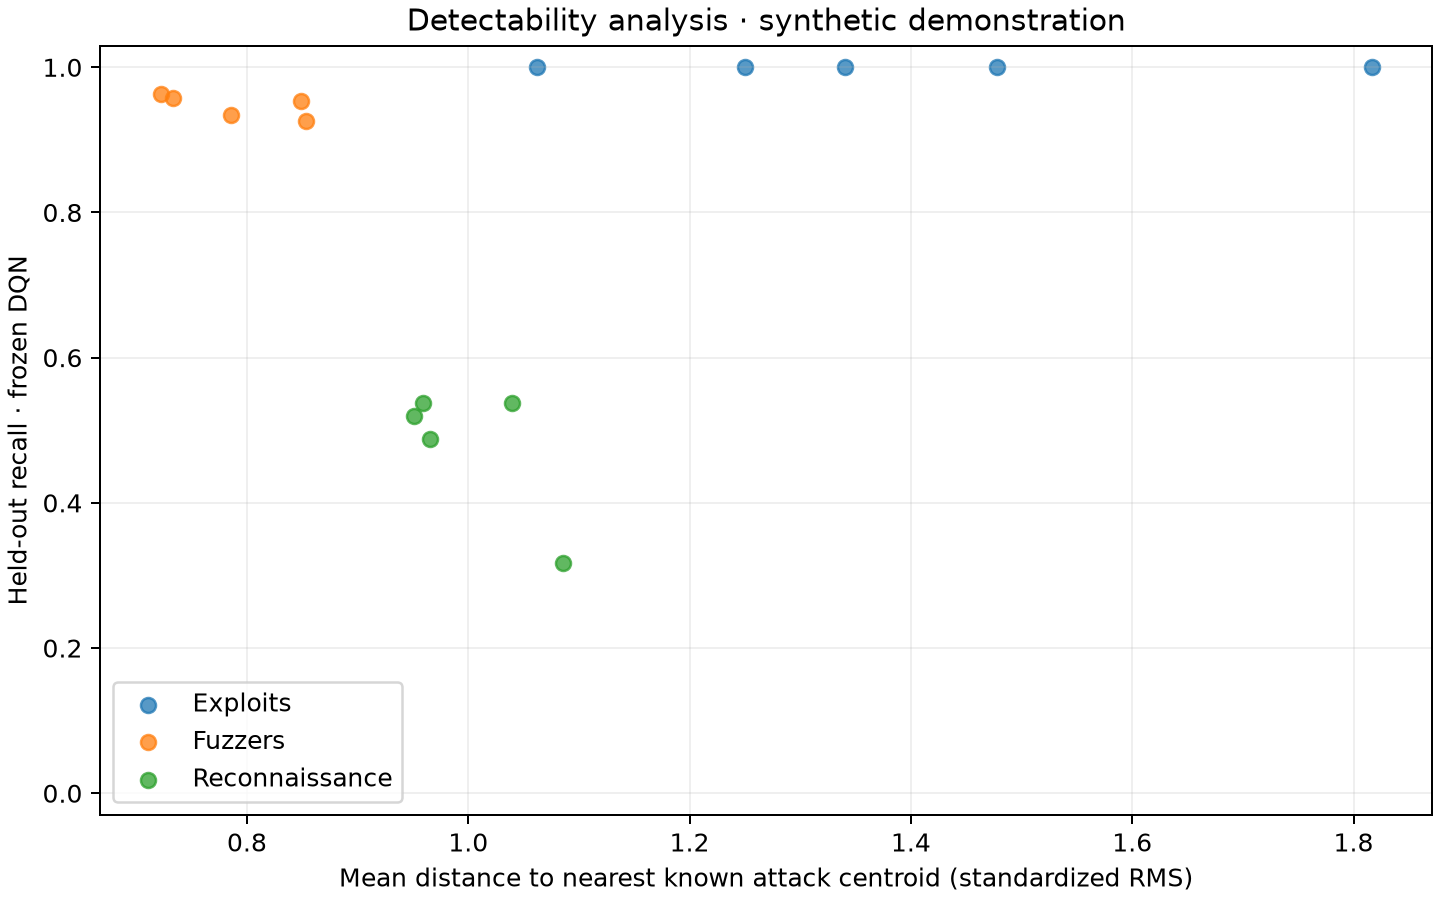
\includegraphics[width=\columnwidth]{detectability.png}\caption{Frozen DQN detectability on synthetic data. Each point is one held-out-family/seed run.}\end{figure}
These results characterize this synthetic generator only. Cross-family distance comparisons are exploratory because each encoder is trained separately.
Reconnaissance had mean distance 1.000 and recall 0.480, compared with Fuzzers
distance 0.789 and recall 0.947. Thus mean centroid distance did not monotonically
order detection performance in this experiment. Random Forest did not perform
worse than the frozen DQN on mean held-out recall for these three families.
On the local Intel CPU, ONNX Runtime 1.24.4 with one thread gave median batch
latencies of 0.0937, 0.2265 and 1.1846 ms at batch sizes 1, 32 and 256.
These are reconstruction-only measurements, not end-to-end detection latency.

\section{Independent Validation Plan}
An internally isolated Docker network contains a disposable HTTP target and a traffic generator with packet capture. Scenarios include browsing, bounded TCP service probes and rejected login requests. Collected flows must use the same feature exporter and semantics as training inputs. Matching column names is insufficient. The local Docker engine was unavailable during preparation, so no external-traffic result is reported.
\section{Usability and Runtime}
A five-participant protocol uses task completion and the unchanged System Usability Scale. No participant scores have been collected. CPU latency measures autoencoder ONNX inference with warm-up, stated thread count and batch sizes; it excludes flow extraction, preprocessing, the controller and API overhead. No Raspberry Pi measurement is claimed.
\section{Limitations}
The synthetic generator creates artificial class separation. Custom stratification is not a chronological or host-independent evaluation. A perfect immediate analyst in the budget simulator is unrealistic. Centroid distances can hide multimodal classes. Publication requires real-data results, uncertainty analysis, independent sessions and author review.
\section{Conclusion}
The contribution is a reproducible evaluation workflow and explicit failure analysis. Real-world detection effectiveness remains an open empirical question.
\begin{thebibliography}{9}
\bibitem{mitre} MITRE, ``Network Service Discovery, T1046,'' \url{https://attack.mitre.org/techniques/T1046/}, accessed October 2026.
\bibitem{sus} J. Brooke, ``SUS: A quick and dirty usability scale,'' in Usability Evaluation in Industry, 1996.
\bibitem{ort} ONNX Runtime, ``Performance and thread management,'' \url{https://onnxruntime.ai/docs/performance/}, accessed October 2026.
\end{thebibliography}
\end{document}
